\chapter{Конструкторская часть}

В данном разделе будут представлены схемы алгоритмов умножения матриц: стандартного алгоритма, алгоритма Винограда и оптимизированного алгоритма Винограда. Будут описаны типы и структуры данных, используемые для реализации, а также структура разрабатываемого программного обеспечения. Кроме того, будут выделены классы эквивалентности для тестирования.

\section{Разработка алгоритмов}

На рисунке \ref{img:standard} приведена схема стандартного алгоритма умножения матриц. 
Схема умножения матриц по алгоритму Винограда приведена на рисунках \ref{img:winograd}-\ref{img:winograd_result}, схема оптимизированной версии приведена на рисунках \ref{img:optimized}-\ref{img:result_optimized}.

\begin{figure}[H]
	\begin{center}
		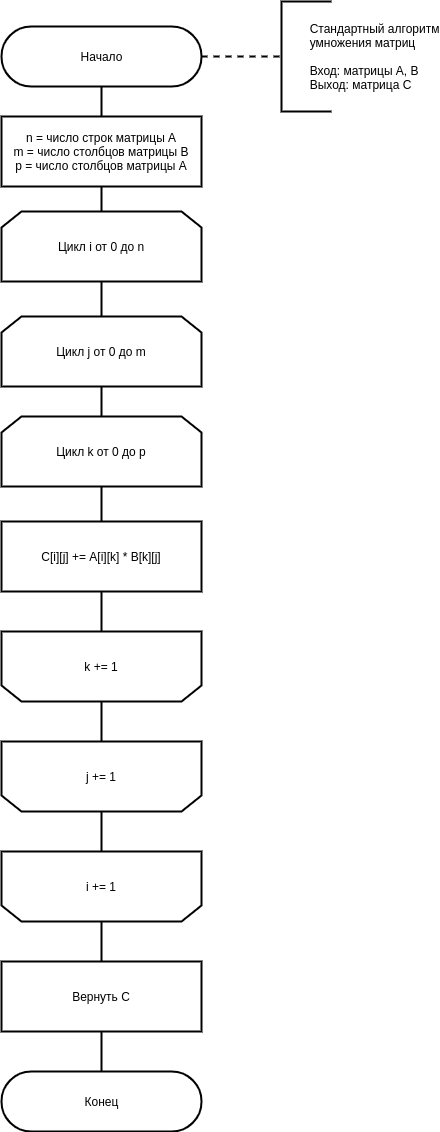
\includegraphics[scale=0.6]{img/standard.png}
	\end{center}
	\captionsetup{justification=centering}
	\caption{Стандартный алгоритм умножения матриц}
	\label{img:standard}
\end{figure}

\begin{figure}[H]
	\begin{center}
		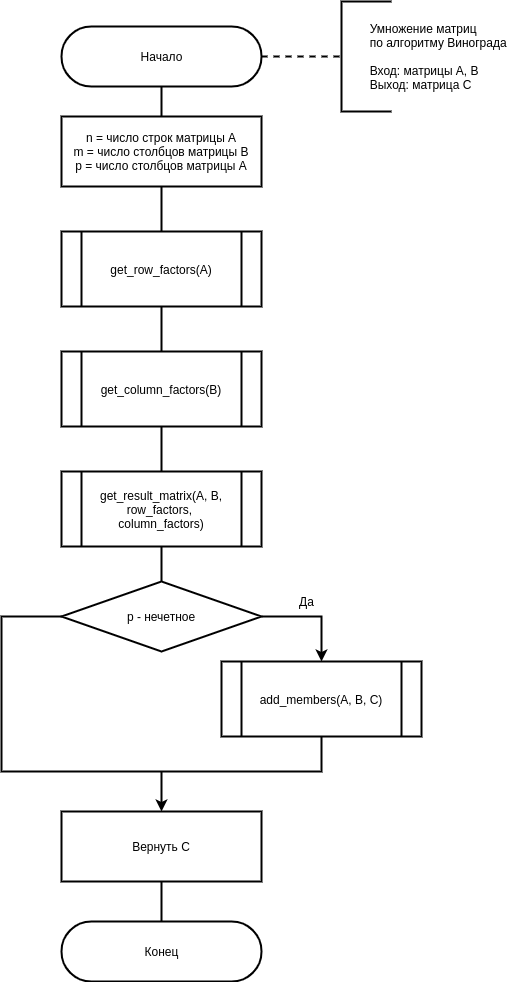
\includegraphics[scale=0.6]{img/winograd.png}
	\end{center}
	\captionsetup{justification=centering}
	\caption{Умножение матриц по алгоритму Винограда}
	\label{img:winograd}
\end{figure}

\begin{figure}[H]
	\begin{center}
		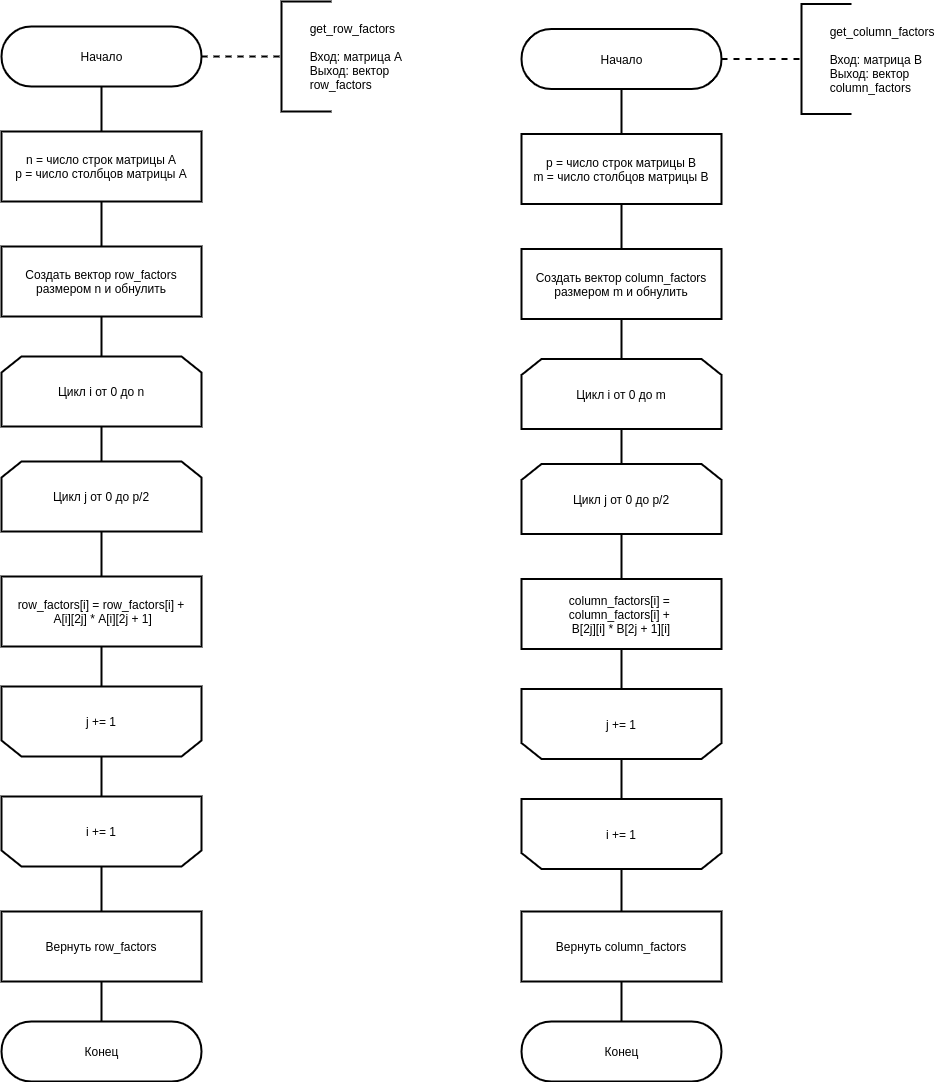
\includegraphics[scale=0.5]{img/factors_winograd.png}
	\end{center}
	\captionsetup{justification=centering}
	\caption{Предварительные вычисления в умножении матриц по алгоритму Винограда}
	\label{img:factors_winograd}
\end{figure}

\begin{figure}[H]
	\begin{center}
		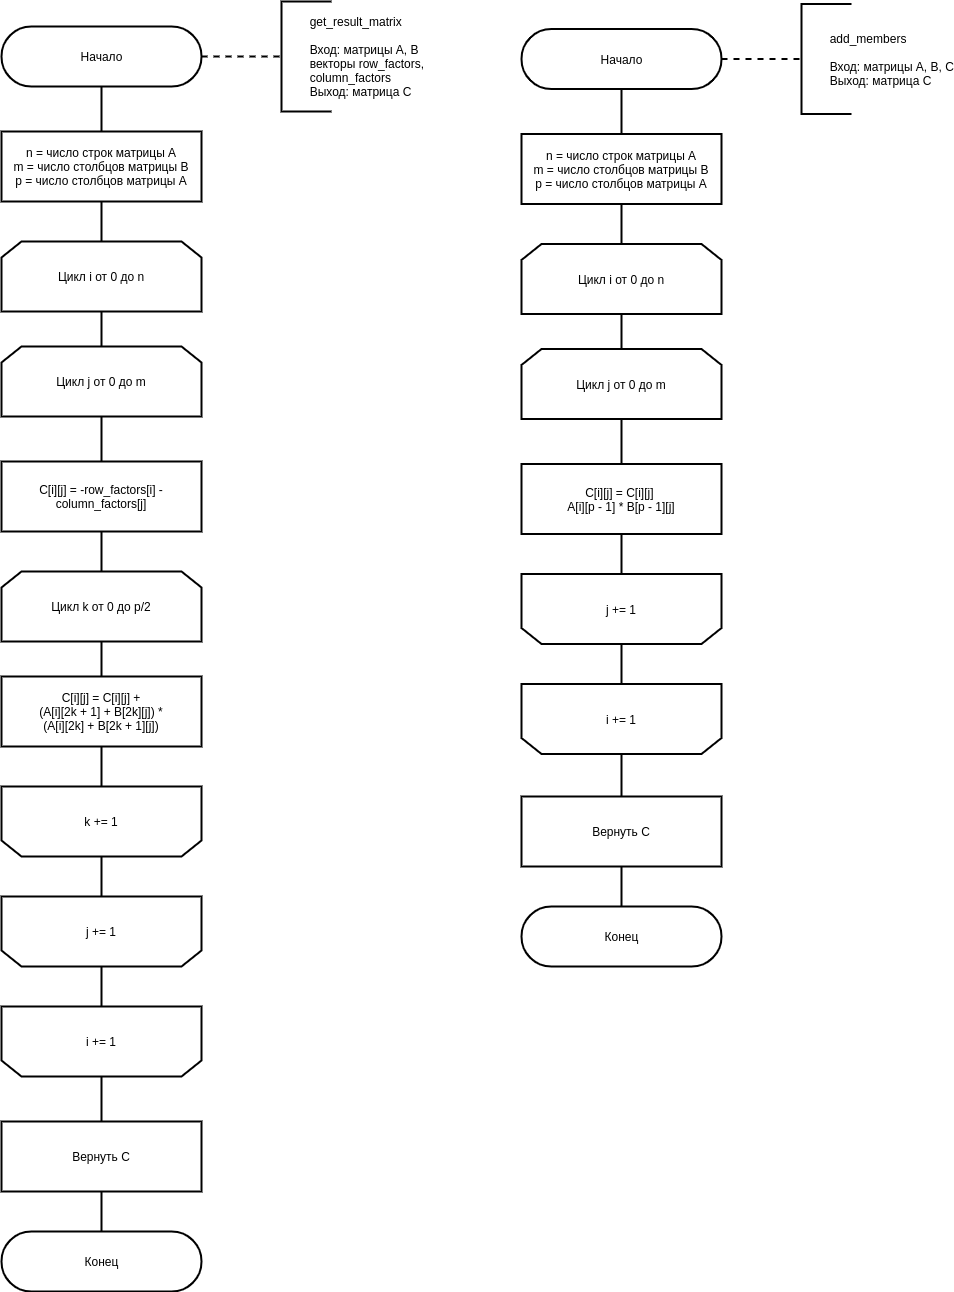
\includegraphics[scale=0.5]{img/winograd_result.png}
	\end{center}
	\captionsetup{justification=centering}
	\caption{Вычисление результата умножения матриц по алгоритму Винограда}
	\label{img:winograd_result}
\end{figure}

\begin{figure}[H]
	\begin{center}
		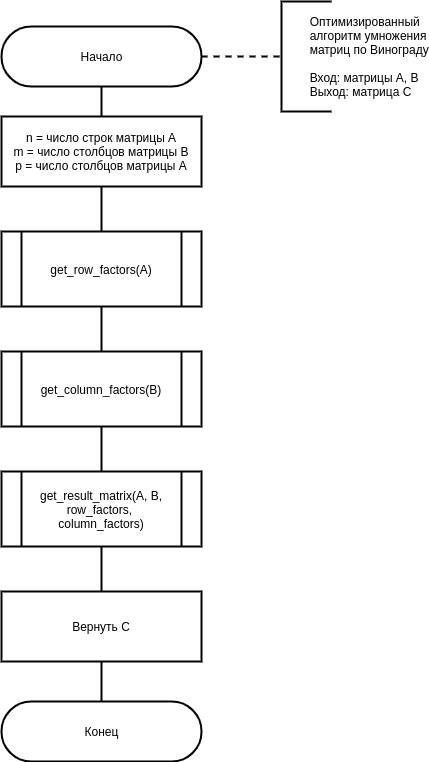
\includegraphics[scale=0.7]{img/optimized_winograd.png}
	\end{center}
	\captionsetup{justification=centering}
	\caption{Умножение матриц по оптимизированному алгоритму Винограда}
	\label{img:optimized}
\end{figure}

\begin{figure}[H]
	\begin{center}
		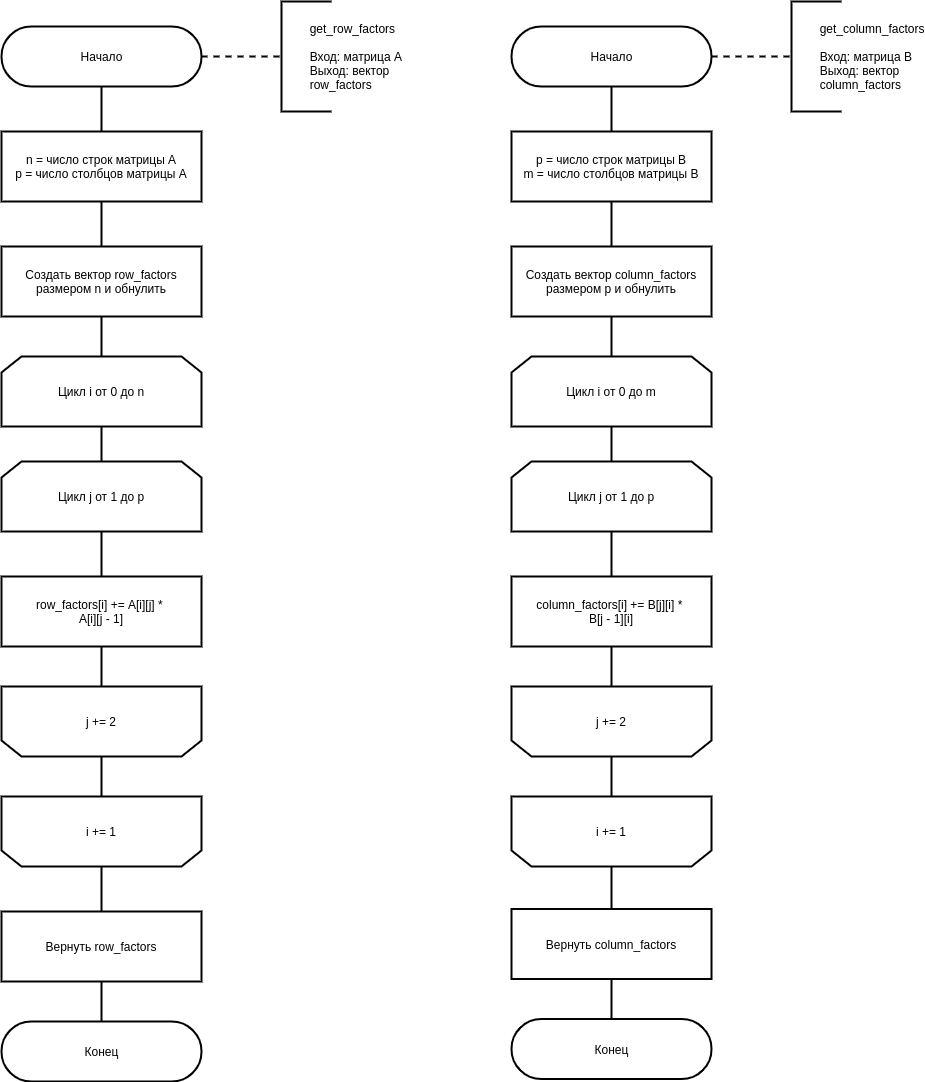
\includegraphics[scale=0.5]{img/factors_optimized.png}
	\end{center}
	\captionsetup{justification=centering}
	\caption{Предварительные вычисления в умножении матриц по оптимизированному алгоритму Винограда}
	\label{img:factors_optimized}
\end{figure}

\begin{figure}[H]
	\begin{center}
		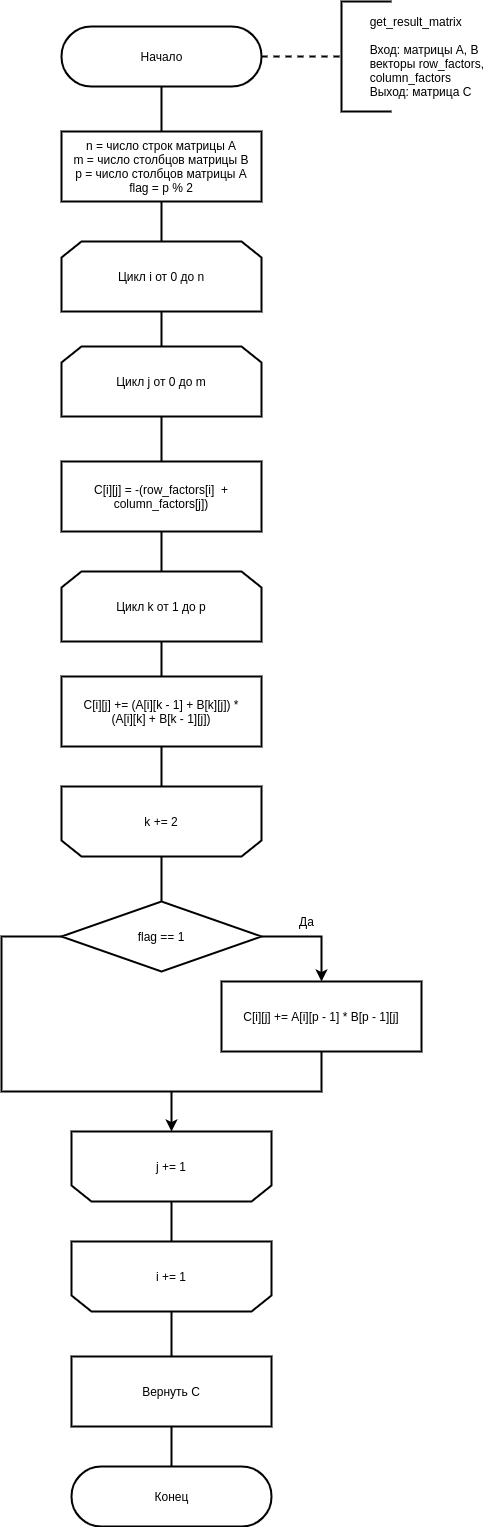
\includegraphics[scale=0.4]{img/result_optimized.png}
	\end{center}
	\captionsetup{justification=centering}
	\caption{Вычисление результата умножения матриц по оптимизированному алгоритму Винограда}
	\label{img:result_optimized}
\end{figure}

\section{Модель вычислений для оценки трудоемкости алгоритмов}

Для определения трудоемкости алгоритмов необходимо ввести модель вычислений \cite{model}:

\begin{enumerate}
	\item операции из списка (\ref{for:operations}) имеют трудоемкость равную 1;
	\begin{equation}
		\label{for:operations}
		+, -, /, *, \%, =, +=, -=, *=, /=, \%=, ==, !=, <, >, <=, >=, [], ++, {-}-
	\end{equation}
	\item трудоемкость оператора выбора \code{if условие then A else B} рассчитывается, как (\ref{for:if});
	\begin{equation}
		\label{for:if}
		f_{if} = f_{\text{условия}} +
		\begin{cases}
			f_A, & \text{если условие выполняется,}\\
			f_B, & \text{иначе.}
		\end{cases}
	\end{equation}
	\item трудоемкость цикла рассчитывается, как (\ref{for:cycle});
	\begin{equation}
		\label{for:cycle}
		f_{for} = f_{\text{инициализации}} + f_{\text{сравнения}} + N(f_{\text{тела}} + f_{\text{инкремент}} + f_{\text{сравнения}})
	\end{equation}
	\item трудоемкость вызова функции равна 0.
\end{enumerate}

\section{Трудоемкость алгоритмов}

Проведем сравнительный анализ реализованных алгоритмов по трудоемкости для умножения матрицы A[N][P] и матрицы B[P][M].

\subsection{Стандартный алгоритм умножения матриц}

Трудоемкость данного алгоритма будет складываться из:

\begin{itemize}
	\item трудоемкости цикла по $k \in [0..P-1]$, равной $1 + P(3 + 8) = 1 + 11P$;
	\item трудоекмости цикла по $j \in [0..M-1]$, равной $1 + M(3 + f_{body}) = 1 + M(3 + 1 + 11P) = 1 + 4M + 11PM$;
	\item трудоемкости цикла по $i \in [0..N-1]$, равной $1 + N(3 + f_{body}) = 1 + N(3 + 1 + 4M + 11MP) = 1 + 4N + 4NM + 11NMP$.
\end{itemize}

Таким образом, трудоемкость стандартного алгоритма умножения равна $f_{standard} = 1 + 4N + 4NM + 11NMP \approx 11NMP$.

\subsection{Алгоритм умножения матриц по Винограду}

Трудоемкость данного алгоритма будет складываться из:

\begin{itemize}
	\item трудоемкости создания и заполнения нулями векторов row\_factors и column\_factors, равной $N + M$;
	\item трудоемкости предварительных вычислений для строк, равной $1 + N(3 + 1 + P/2(3 + 12)) = 1 + 4N + 7.5NP$;
	\item трудоемкости предварительных вычислений для столбцов, равной $1 + M(3 + 1 + P/2(3 + 12)) = 1 + 4M + 7.5MP$;
	\item трудоемкости цикла по $k \in [0..P/2-1]$, равной $1 + P/2(3 + 23) = 1 + 13P$;
	\item трудоекмости цикла по $j \in [0..M-1]$, равной $1 + M(3 + f_{body}) = 1 + M(3 + 7 + 1 + 13P) = 1 + 11M + 13PM$;
	\item трудоемкости цикла по $i \in [0..N-1]$, равной $1 + N(3 + f_{body}) = 1 + N(3 + 1 + 11M + 13MP) = 1 + 4N + 11NM + 13NMP$;
	\item трудоемкости условия, равной $2$;
	\item трудоемкости двойного цикла добавления в случае нечетного размера матрицы, равной $1 + N(3 + 1 + M(3 + 13)) = 1 + 4N + 16NM$.
\end{itemize}

Таким образом, трудоемкость алгоритма умножения по Винограду в худшем случае (нечетный размер матрицы) равна $f_{worst} = N + M + 2(1 + 4N + 7.5M) + 1 + 4N + 11NM + 13NMP + 2 + 1 + 4N + 16NM = 6 + 17N + 16M + 27NM + 13NMP \approx 13NMP$.

Трудоемкость алгоритма умножения по Винограду в лучшем случае (четный размер матрицы) равна $f_{best} = N + M + 2(1 + 4N + 7.5M) + 1 + 4N + 11NM + 13NMP + 2 = 5 + 13N + 16M + 11NM + 13NMP \approx 13NMP$.

\subsection{Оптимизированный алгоритм умножения матриц по Винограду}

Трудоемкость данного алгоритма будет складываться из:

\begin{itemize}
	\item трудоемкости создания и заполнения нулями векторов row\_factors и column\_factors, равной $N + M$;
	\item трудоемкости предварительных вычислений для строк, равной $1 + N(3 + 1 + P/2(3 + 8)) = 1 + 4N + 5.5NP$;
	\item трудоемкости предварительных вычислений для столбцов, равной $1 + M(3 + 1 + P/2(3 + 8)) = 1 + 4M + 5.5MP$;
	\item трудоемкости вычисления признака четности размера матрицы, равной $2$;
	\item трудоемкости цикла по $k \in [0..P/2-1]$, равной $1 + P/2(3 + 16) = 1 + 9.5P$;
	\item трудоемкости условия, равной $1$;
	\item трудоемкости добавления в случае нечетного размера матрицы, равной $10$;
	\item трудоекмости цикла по $j \in [0..M-1]$, равной $1 + M(3 + f_{body})$;
	\item трудоемкости цикла по $i \in [0..N-1]$, равной $1 + N(3 + f_{body})$.
\end{itemize}

Таким образом, трудоемкость оптимизированного алгоритма умножения по Винограду в худшем случае (нечетный размер матрицы) равна $f_{worst} = N + M + 2(1 + 4N + 5.5M) + 2 + 1 + N(3 + 1 + M(3 + 7 + 1 + 9.5P + 1 + 10)) = 5 + 13N + 12M + 22MN + 9.5MNP \approx 9.5NMP$.

Трудоемкость оптимизированного алгоритма умножения по Винограду в лучшем случае (четный размер матрицы) равна $f_{best} = N + M + 2(1 + 4N + 5.5M) + 2 + 1 + N(3 + 1 + M(3 + 7 + 1 + 9.5P + 1)) = 5 + 13N + 12M + 11MN + 9.5MNP \approx 9.5NMP$.


\section{Описание используемых типов и структур данных}

Для реализации рассмотренных алгоритмов будет использован тип данных $int$ - для числа строк и числа столбцов каждой матрицы.

Структура данных - матрица - представляет собой двумерный список значений типа $int$.

\section{Структура разрабатываемого ПО}

При реализации разрабатываемого программного обеспечения будет использоваться метод структурного программирования. Для взаимодействия с пользователем будет выделена функция process(), из которой будут вызываться методы умножения матриц и функции сравнительного анализа. Для работы с матрицами будут разработаны следущие функции:

\begin{itemize}
	\item создание матрицы случайных чисел, входным параметром функции является размер, выходным - матрица;
	\item ввод матрицы, функция не имеет входных параметров, выходным параметром является введенная матрица;
	\item процедура вывода матрицы, входным параметром которой является матрица;
	\item функции умножения матриц для каждого алгоритма (классического, Винограда и оптимизированного Винограда), у которых на входе - две матрицы для умножения, а на выходе - результат умножения матриц. 
\end{itemize}

Для сравнительного анализа будут реализованы:

\begin{itemize}
	\item процедура замеров времени, выходным парметром которой является массив временных значений;
	\item функция графического представления замеров времени, у которой на входе - массив временных значений, на выходе - его графическое представление.
\end{itemize}

\section{Классы эквивалентности при тестировании}

Для тестирования разрабатываемой программы будут выделены следующие классы эквивалентности:

\begin{itemize}
	\item две пустые матрицы;
	\item одна пустая матрица, одна нет;
	\item число столбцов первой матрицы не равно числу строк второй;
	\item умножение квадратных матриц;
	\item умножение матриц с одинаковым числом стоблцов первой и числом строк второй, но разным числом строк первой и числом столбцов второй.
\end{itemize}

\section{Вывод}

Были представлены схемы алгоритмов умножения матриц. Были указаны типы и структуры данных, используемые для реализации, и описана структура разрабатываемого программного обеспечения. Также были выделены классы эквивалентности для тестирования ПО.
